\section{Results and Discussion}\label{sec:result}


Based on the two-step approach of folding a carton model as well as the suggestive user interface, our system is natural and easy to use. 
%
We will show a series of results of cartons in various shapes. 
%
\reply{A user study was also conducted to examine the effectivenss of our suggestive system.}

\subsection{Carton Results}

%%%%%%%%%%% Fully automatic results %%%%%%%%%%%

For most cuboid cartons, their 3D models can be generated by folding each edge by $\pi/2$, as shown in Figure~\ref{fig:initial-automatic} and Figure~\ref{fig:automatic-more}.
In the common design process nowadays, designers typically spend much time on manually creating the 3D carton models in 3D modeling softwares. 
Our suggestive interface significantly saves the designers' effort so that they can focus on the appearance designing of cartons. 


\begin{figure}
	\centering
	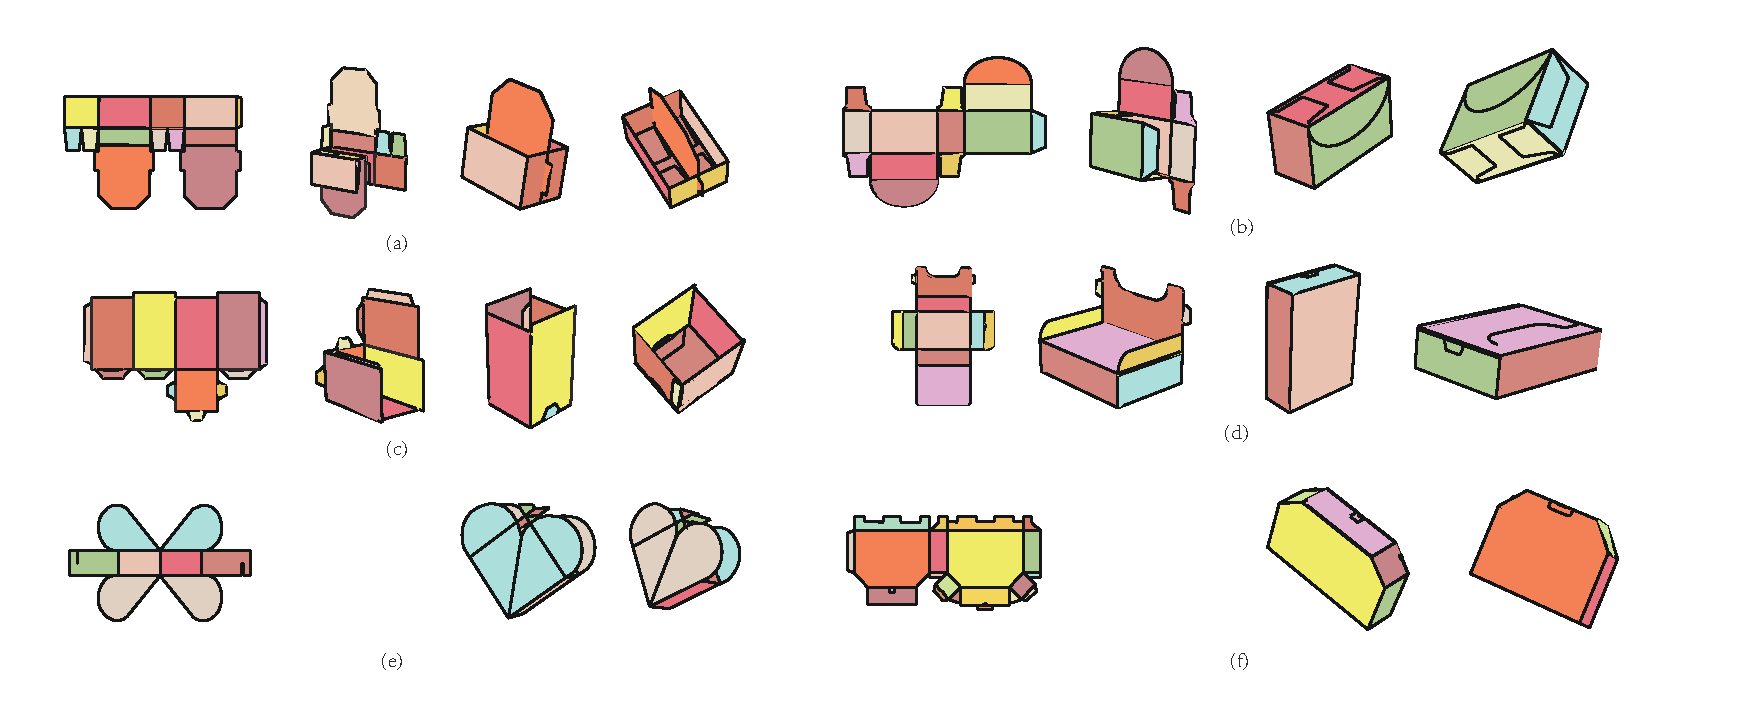
\includegraphics[width=\textwidth]{images/moreAutomatic}
	\caption{More carton examples that can be automatically generated. \xjmd{For each example, four subfigures are shown from left to right: the input 2D layout, an intermediate stage during folding, and the final 3D shape at two different views.}  }
	\label{fig:automatic-more}
	
\end{figure}

%%%%%%%%%% Results with refinement %%%%%%%%%%

For more complicated cartons, shape refinement is required. 
An entire process of creating a carton model from a 2D layout is illustrated in Figure~\ref{fig:result}.
%
The final model can be generated by three clicks from the user to confirm vertex merging two times, and \cxj{face pasting} in one time.
\reply{Note that our system automatically detects these possible geometric editing options for users to select. Therefore, the user can get rid of the tedious work of selecting edges or vertexes and assigning precise length or positions to them.}
%
A more challenging example is shown in Figure~\ref{fig:hexagon}. 
By initially folding each edge as $\pi/2$, our system firstly generates a cube inside the carton for the six square faces. 
Sometimes, our system fails to detect mergeable vertexes with a small threshold $\epsilon$ to merge closeby vertexes.
%
However, the user could manually select two vertexes to merge. Then our systems automatically detects two symmetric vertexes that also can be merged. 
%
Finally, a hexagonal carton can be generated in a limited number of user interactions.
%


\begin{figure}
	\centering
	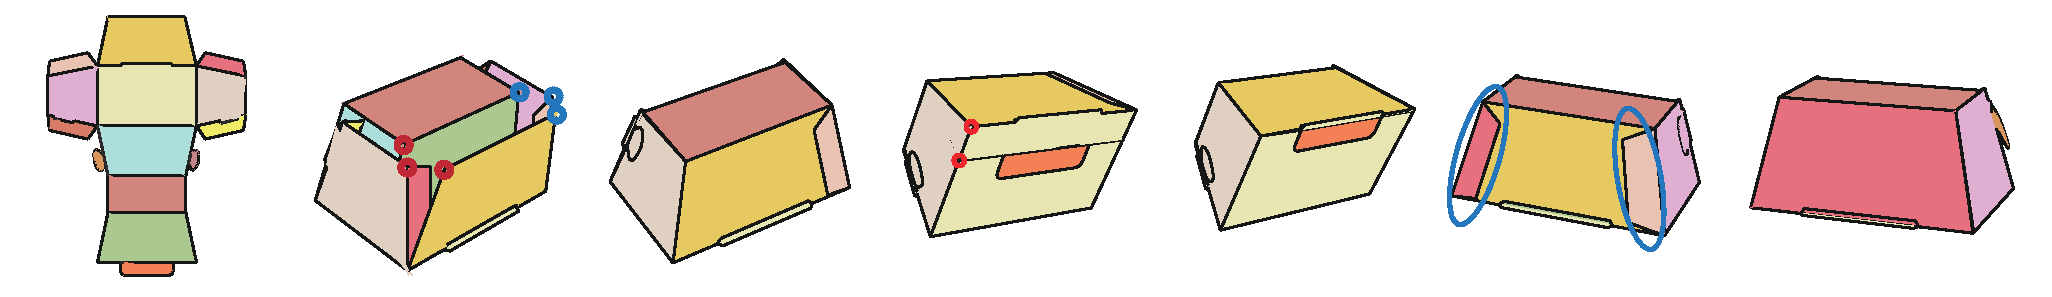
\includegraphics[width=\textwidth]{images/105}
	\caption{Structural layout is used to generate flat polymesh, and then initialize to a rough model, after two vertex merging confirmations and one face pasting confirmation, we can finally have its corresponding 3D model.}
	\label{fig:result}
\end{figure}
%





\begin{figure}
	\centering
	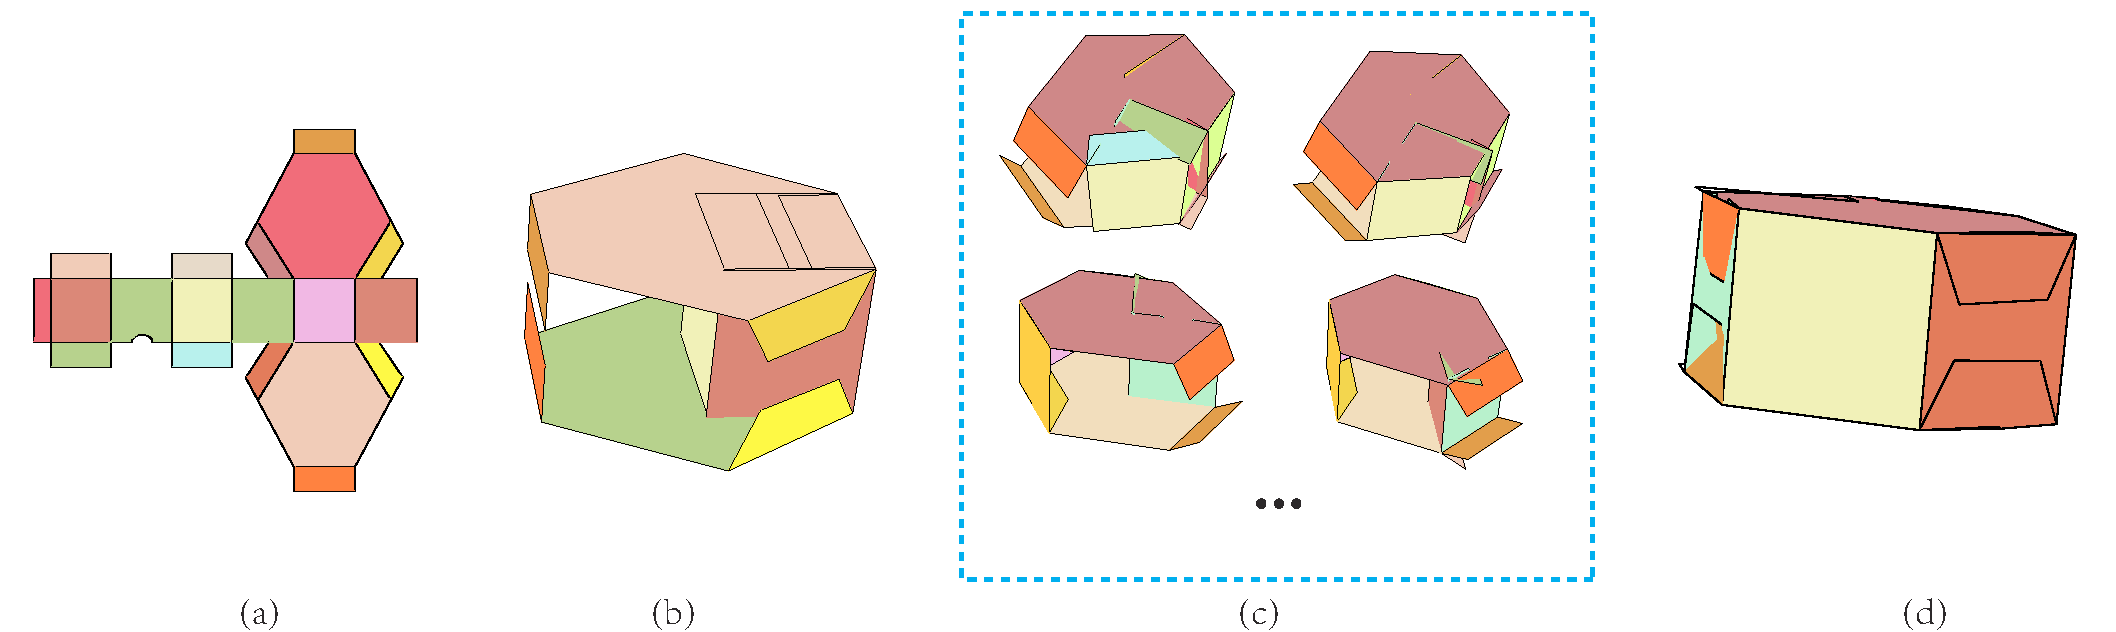
\includegraphics[width=0.9\textwidth]{images/limitation}
	\caption{Given a layout as (a), our system can generate an initialized result as (b), and through almost ten steps including selecting merging vertexes and faces need to be coplane , users can reach the final model as (d). }
	\label{fig:hexagon}
\end{figure}


\begin{figure}
	\centering
	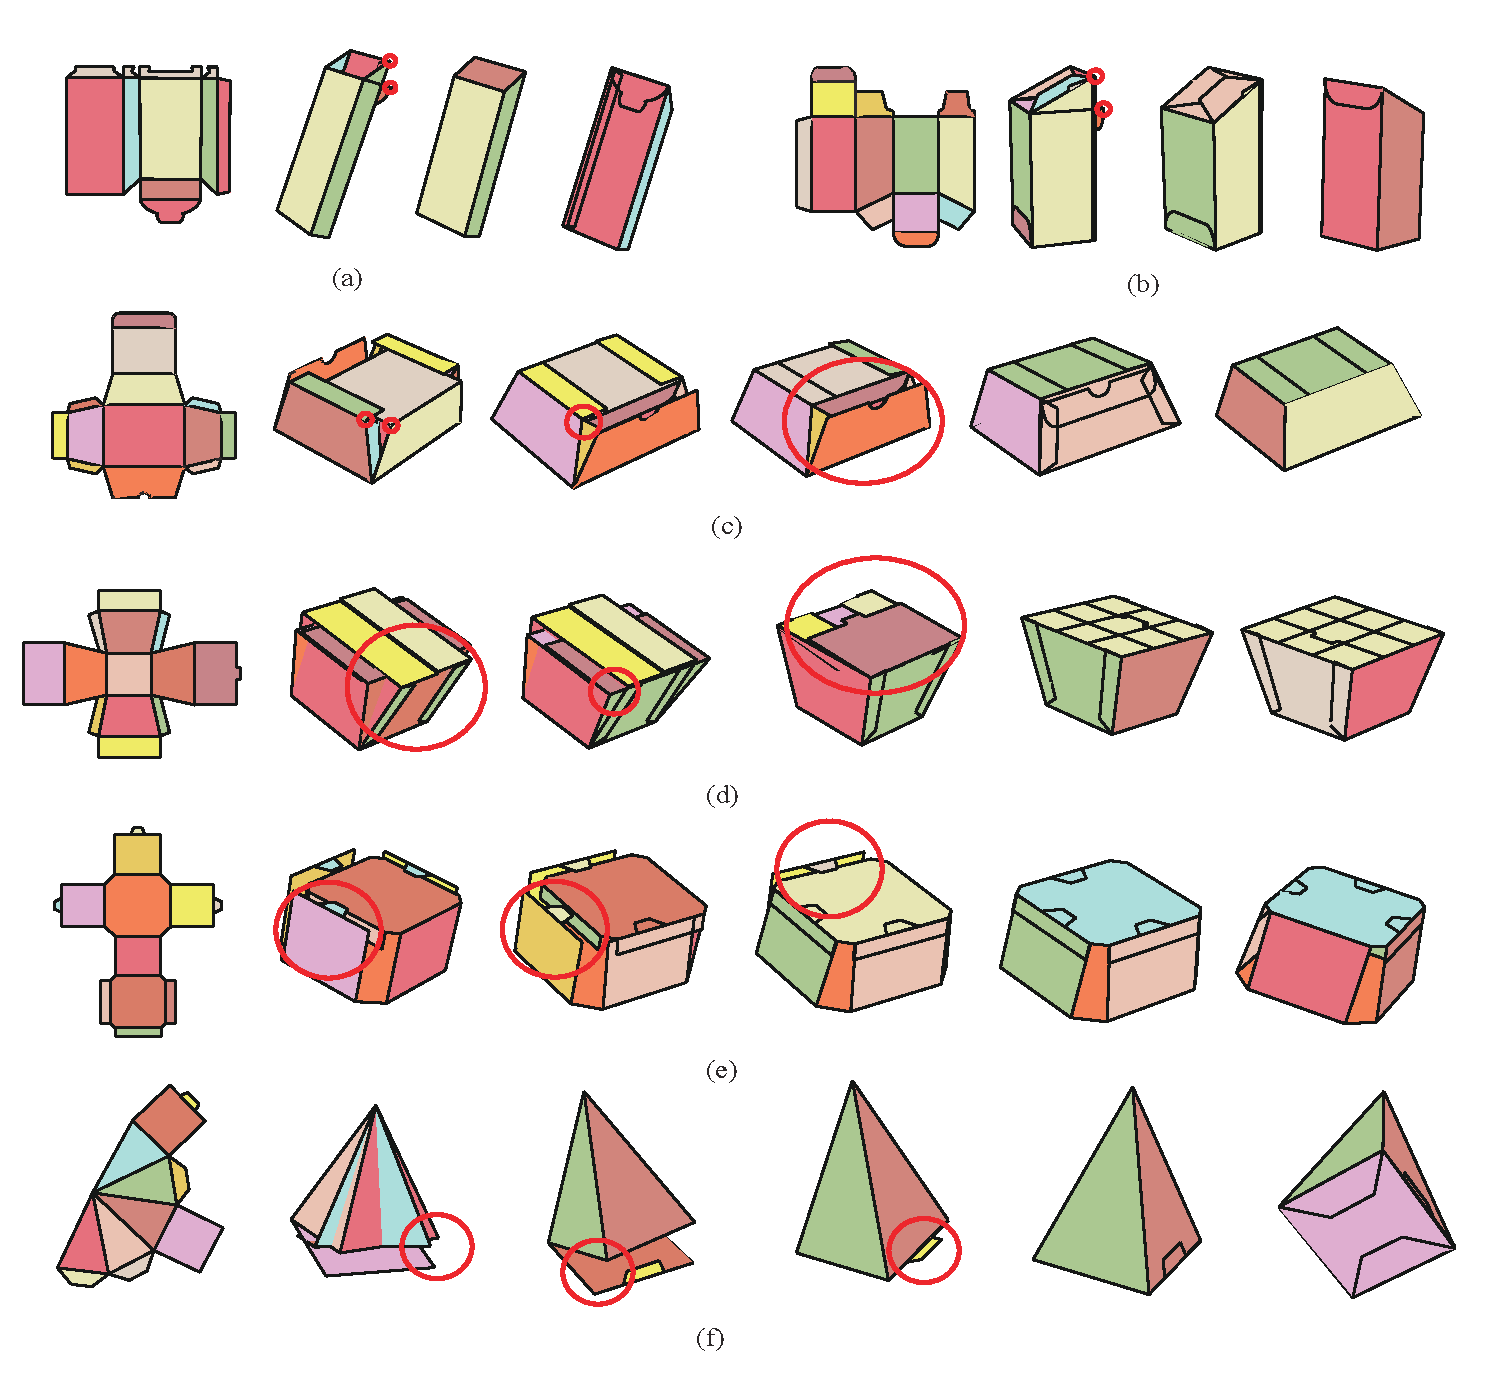
\includegraphics[width=0.9\textwidth]{images/newMore}
	\caption{More results need refinement. Users can manipulate more complicated cartons. The first and second column in each sub-figure are the flat mesh and initialization result of cartons, and the last two column shows the model after interaction in  different views. Circles marked in red means the part that need to be merged.}
	\label{fig:result-more}
\end{figure}



More carton models generated using our system \xjmd{with a few user interactions} are shown in Figure~\ref{fig:result-more}.
The statistics of the face number, edge number, and number of user interactions are listed in Table~\ref{table:statistics}. 
We can see that only a few user interactions on confirming system suggestions are needed for a variety of shapes.


\begin{table}
	\centering
	\caption{Statistics on the number of edges $N_{edge}$, number of faces $N_{face}$, and the number of user interactions $N_{interaction}$ of the examples shown in this paper.}
	\setlength{\tabcolsep}{1pt}
	\begin{tabular}{c|c|c|c|c|c|c|c|c|c|c|c|c}
		\hline
		Examples & Fig.\ref{fig:automatic-more}(a) & Fig.\ref{fig:automatic-more}(b) &  Fig.\ref{fig:automatic-more}(c) & Fig.\ref{fig:automatic-more}(d) & Fig.\ref{fig:result} & Fig.\ref{fig:hexagon} & Fig.\ref{fig:result-more}(a) & Fig.\ref{fig:result-more}(b)& Fig.\ref{fig:result-more}(c) &  Fig.\ref{fig:result-more}(d) & Fig.\ref{fig:result-more}(e)& Fig.\ref{fig:result-more}(f)\\
		\hline
		$N_{edge}$ & 49 & 62 & 46 & 45 & 54 & 67 & 40 & 43 & 42 & 38 & 48 & 30\\
		$N_{face}$  & 13 & 13 & 11 & 13 & 14 & 19 & 11 & 13 & 13 & 13 & 12 & 11\\
		$N_{interaction}$  & 0 & 0 & 0 & 0 & 3 & 9 & 1 & 4 & 1 & 3 & 3 & 3\\ 
		\hline
		\end{tabular}
		\label{table:statistics}
\end{table}


%%%%%%% User Study %%%%%%%%%%%%%%%%%%%%%%%%%%%%%
\subsection{User Study}

 
 
 \begin{figure}  
 	\centering
 	\subfigure[System Preference]{
 		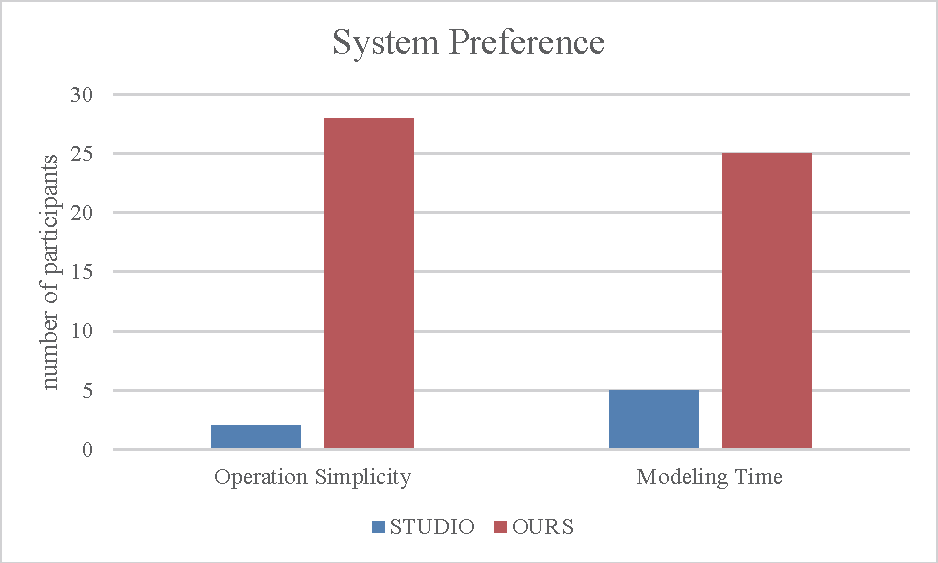
\includegraphics[width=0.25\columnwidth,height=0.11\textheight]{images/preference}
 		\label{fig:preference}
 	}
 	\vspace{2ex}
 	\subfigure[Layout Refinment]{
 		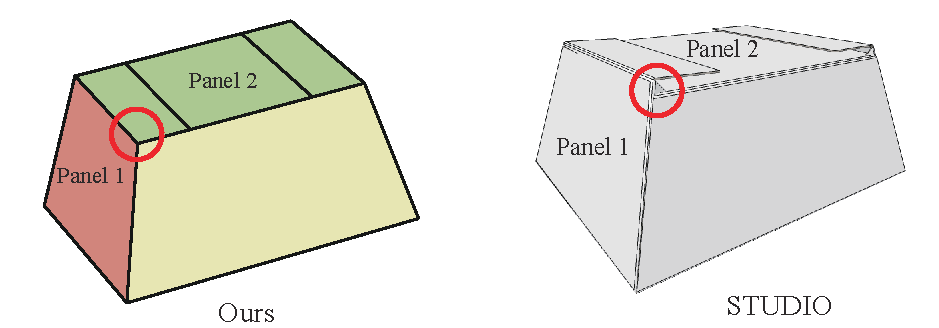
\includegraphics[width=0.35\columnwidth,height=0.08\textheight]{images/comparison}
 		\label{fig:correction}
 	}
 	\vspace{2ex}
 	\subfigure[Fabrication Time]{
 		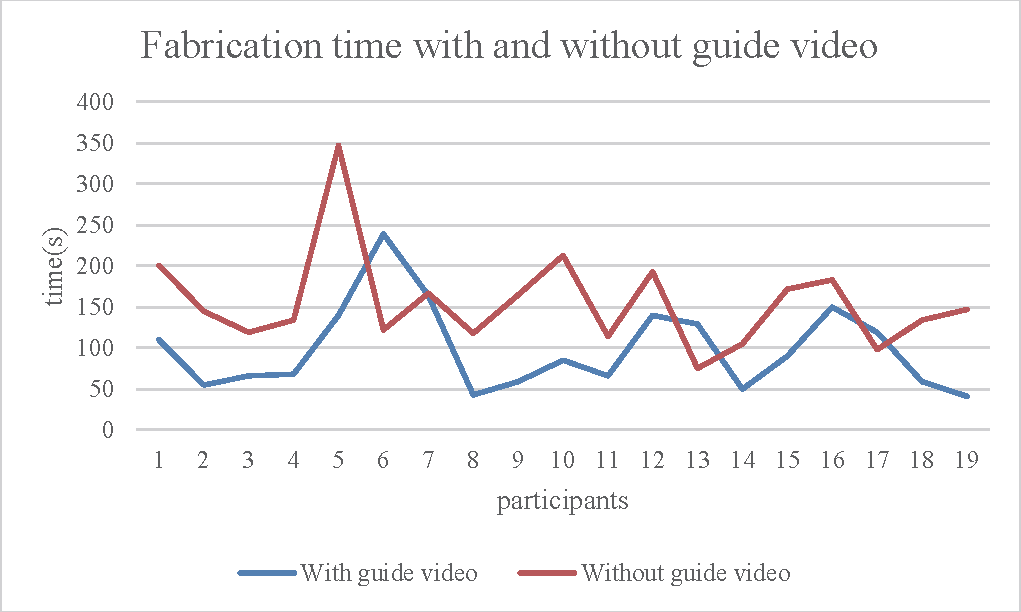
\includegraphics[width=0.25\columnwidth,height=0.11\textheight]{images/fabrication}
 		\label{fig:time}
 	}
 	\caption{(a) Compared with STUDIO, more participants prefer our system with regard to both the operation simplicity and modeling time. (b) Our system is able to automatically refine the inaccurate 2D layout, while STUDIO only generates the folded shape based on user assigned angles. (c) Comparison of fabrication times with/without video. It took much longer for common users to fabricate a carton from a 2D layout without our guide.}
 	\label{fig:userstudy}
 \end{figure}
 
 
 
We conducted a user study to examine the productivity of our system for constructing digital 3D mockups from 2D layouts and to analyze the effectiveness of our system in guiding non-expert users to fabricate physical mockups from 2D layouts. 
%
There are two experiments in our user study.
% 
In the first experiment, participants were given a brief introduction, and then they were asked to construct a digital 3D model from the same 2D layout using our system and the commercial software, STUDIO, respectively.
For each participant, 10 examples were randomly selected from the 34 2D design layouts and presented to the participant for folding using our system and STUDIO.
A \emph{two-alternative forced choices} design was used, so the participant was asked to choose which of the two systems they would prefer to use after considering operation simplicity and modeling efficiency. 
%
Furthermore, participants were asked to rate the necessity of layout optimization in our system by using a scale from one to five, with five indicating that it is very necessary.

%
In the second experiment, participants were separated equally into two groups. One group was asked to fold a sheet of paper into a physical carton. The 2D layout was printed onto this piece of paper, and the user was guided by a video showing the folding sequence according to our system. Another group was asked to make a carton without the guide video. 
Each participant was assigned with the same 2D layout (Figure~\ref{fig:automatic-more}(a)), because it is not easy to imagine the final mockup from the 2D layout at first sight.
%
The fabrication times were recorded for the two groups.
%

Based on the two experiments, our goal was to test the following hypotheses:

\begin{itemize}
	\item \textbf{Hypo1:} Our system takes less time and effort to construct a digital 3D mockup than the traditional software.
	\item \textbf{Hypo2:} Our system provides novel and practical functions for generating diverse layouts.
	\item \textbf{Hypo3:} Our system is effective for guiding non-expert users to fabricate complex cartons from 2D layouts.
\end{itemize}




We consider our three hypotheses in turn. 
With respect to \textbf{Hypo1}, we collect the answers to the former two questions from 30 participants, all over eighteen years of age. Both male and female participants were included, and none had any prior experience with designing or folding cartons in computer software. 
%
The results are shown in Figure~\ref{fig:preference}. 
The chart shows that $93\%$ of participants prefer our system with regard to the operation simplicity, and $83\%$ of participants prefer our system with regard to the modeling time.
%
We also performed a paired-samples $t$-test at the level $\alpha = 0.05$ to compare the preference significance.
%
This test shows that our system is significantly preferred by participants.
%
Most participants voted for our system because it takes much less time to make a 3D model using our system. 
Take Figure~\ref{fig:result-more}(e) for example, participants usually spent much time adjusting the folding angles of the creases, while only three clicks are required in our system.
%
On the other hand, one comment from the participants who preferred STUDIO stated that the operation in STUDIO only required them to select and assign angles, while our system required them to learn more operations to construct the digital 3D model. 
%

With respect to \textbf{Hypo2}, 24 participants gave the highest score to our layout optimization function. 
%
In addition to exploring the diversity of 2D layouts, our system can also adjust the imprecise panels on the 2D layout to reach an ideal model. Figure~\ref{fig:correction} shows the final models constructed by our system and STUDIO, respectively. As we can see, Panel 1 is higher than Panel 2 in the digital model constructed by STUDIO, because the 2D layout is not as precise as the designer would like. 
%
In comparison, our system is able to correct these design errors by merging the 3D vertexes in different panels, which are circled in red. This step optimizes the corresponding 2D layout.
 
 
Considering \textbf{Hypo3}, 38 participants (19 in each group) were asked to transform the 2D layout shown in Figure~\ref{fig:automatic-more}(a) into a physical carton. 
The comparison of the fabrication times with and without our guide video is shown in Figure~\ref{fig:time}. 
As we can see, most participants who did not watch the guide video spent more time, averaging 155 seconds, to fold a carton than the other group, averaging 99 seconds.
% 
%
We also performed an independent-samples $t$-test at the level $\alpha = 0.05$ to compare the fabrication times. The results show that the guide video is a highly effective tool for non-expert users in fabricating complex cartons. 




\paragraph{Limitations}

%%%%%%%%%% Limitations and discussions %%%%%%%%%%%%%%%%%%%%%%%%%%%%%%%%%

\reply{
	Shape optimization can be used in most cases through interaction, however, there are still some failure cases that we can not deal with. Figure~\ref{fig:failure} shows a case that failed to generate 3D model by optimization. The faces circled in red should be merged together to produce a strong enforced face, while our system expanded the face away. Moreover, we cannot deal with the case that if we want to layout down the back red face and keep the bottom lines of green side faces together. The carton layouts whose face graph has a loop will also be failed to construct corresponding model such as milk cartons.  
}

\begin{figure}
	\centering
	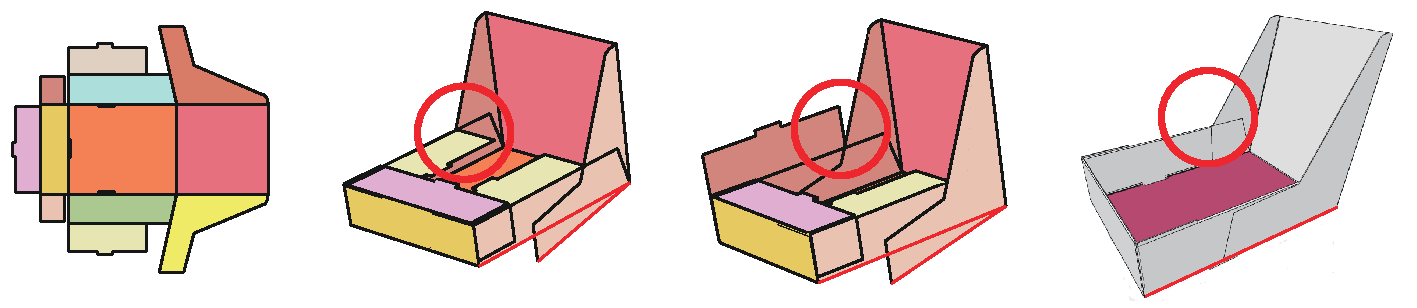
\includegraphics[width=0.9\textwidth]{images/moreLimitation}
	\caption{A failure case that shape optimization can not handle with. }
	\label{fig:failure}
\end{figure}
